%% 第七章 仿真闭环系统与域微调
\chapter{仿真闭环系统与域微调}

在真实空域中开展反无人机实验受到法规、成本与安全的多重限制，因此本文首先在仿真环境中构建闭环验证平台。本章介绍 PX4 SITL 与 jMAVSim 的组合架构、本文对 jMAVSim 的深度改造、仿真场景的构建方法，详细分析检测死区的发现过程与形成机理，给出仿真域微调的完整流程与结果，并介绍目标机主动飞行、相机被动尾随的编队巡游实现。

\section{仿真闭环总体架构}

\subsection{进程与数据流}

仿真闭环由三个进程组成，如图~\ref{fig:sim_arch} 所示。

（1）\textbf{PX4 SITL}：运行飞控固件，负责目标机的姿态控制与位置估计；通过 MAVLink 与 jMAVSim 交换传感器与执行器数据。

（2）\textbf{jMAVSim}：运行三维场景与动力学，负责渲染护航相机画面、广播目标真值、推送视频帧。

（3）\textbf{算法端}：接收视频帧与真值，执行检测、跟踪、定位，输出结构化结果。

\begin{figure}[htbp]
\centering
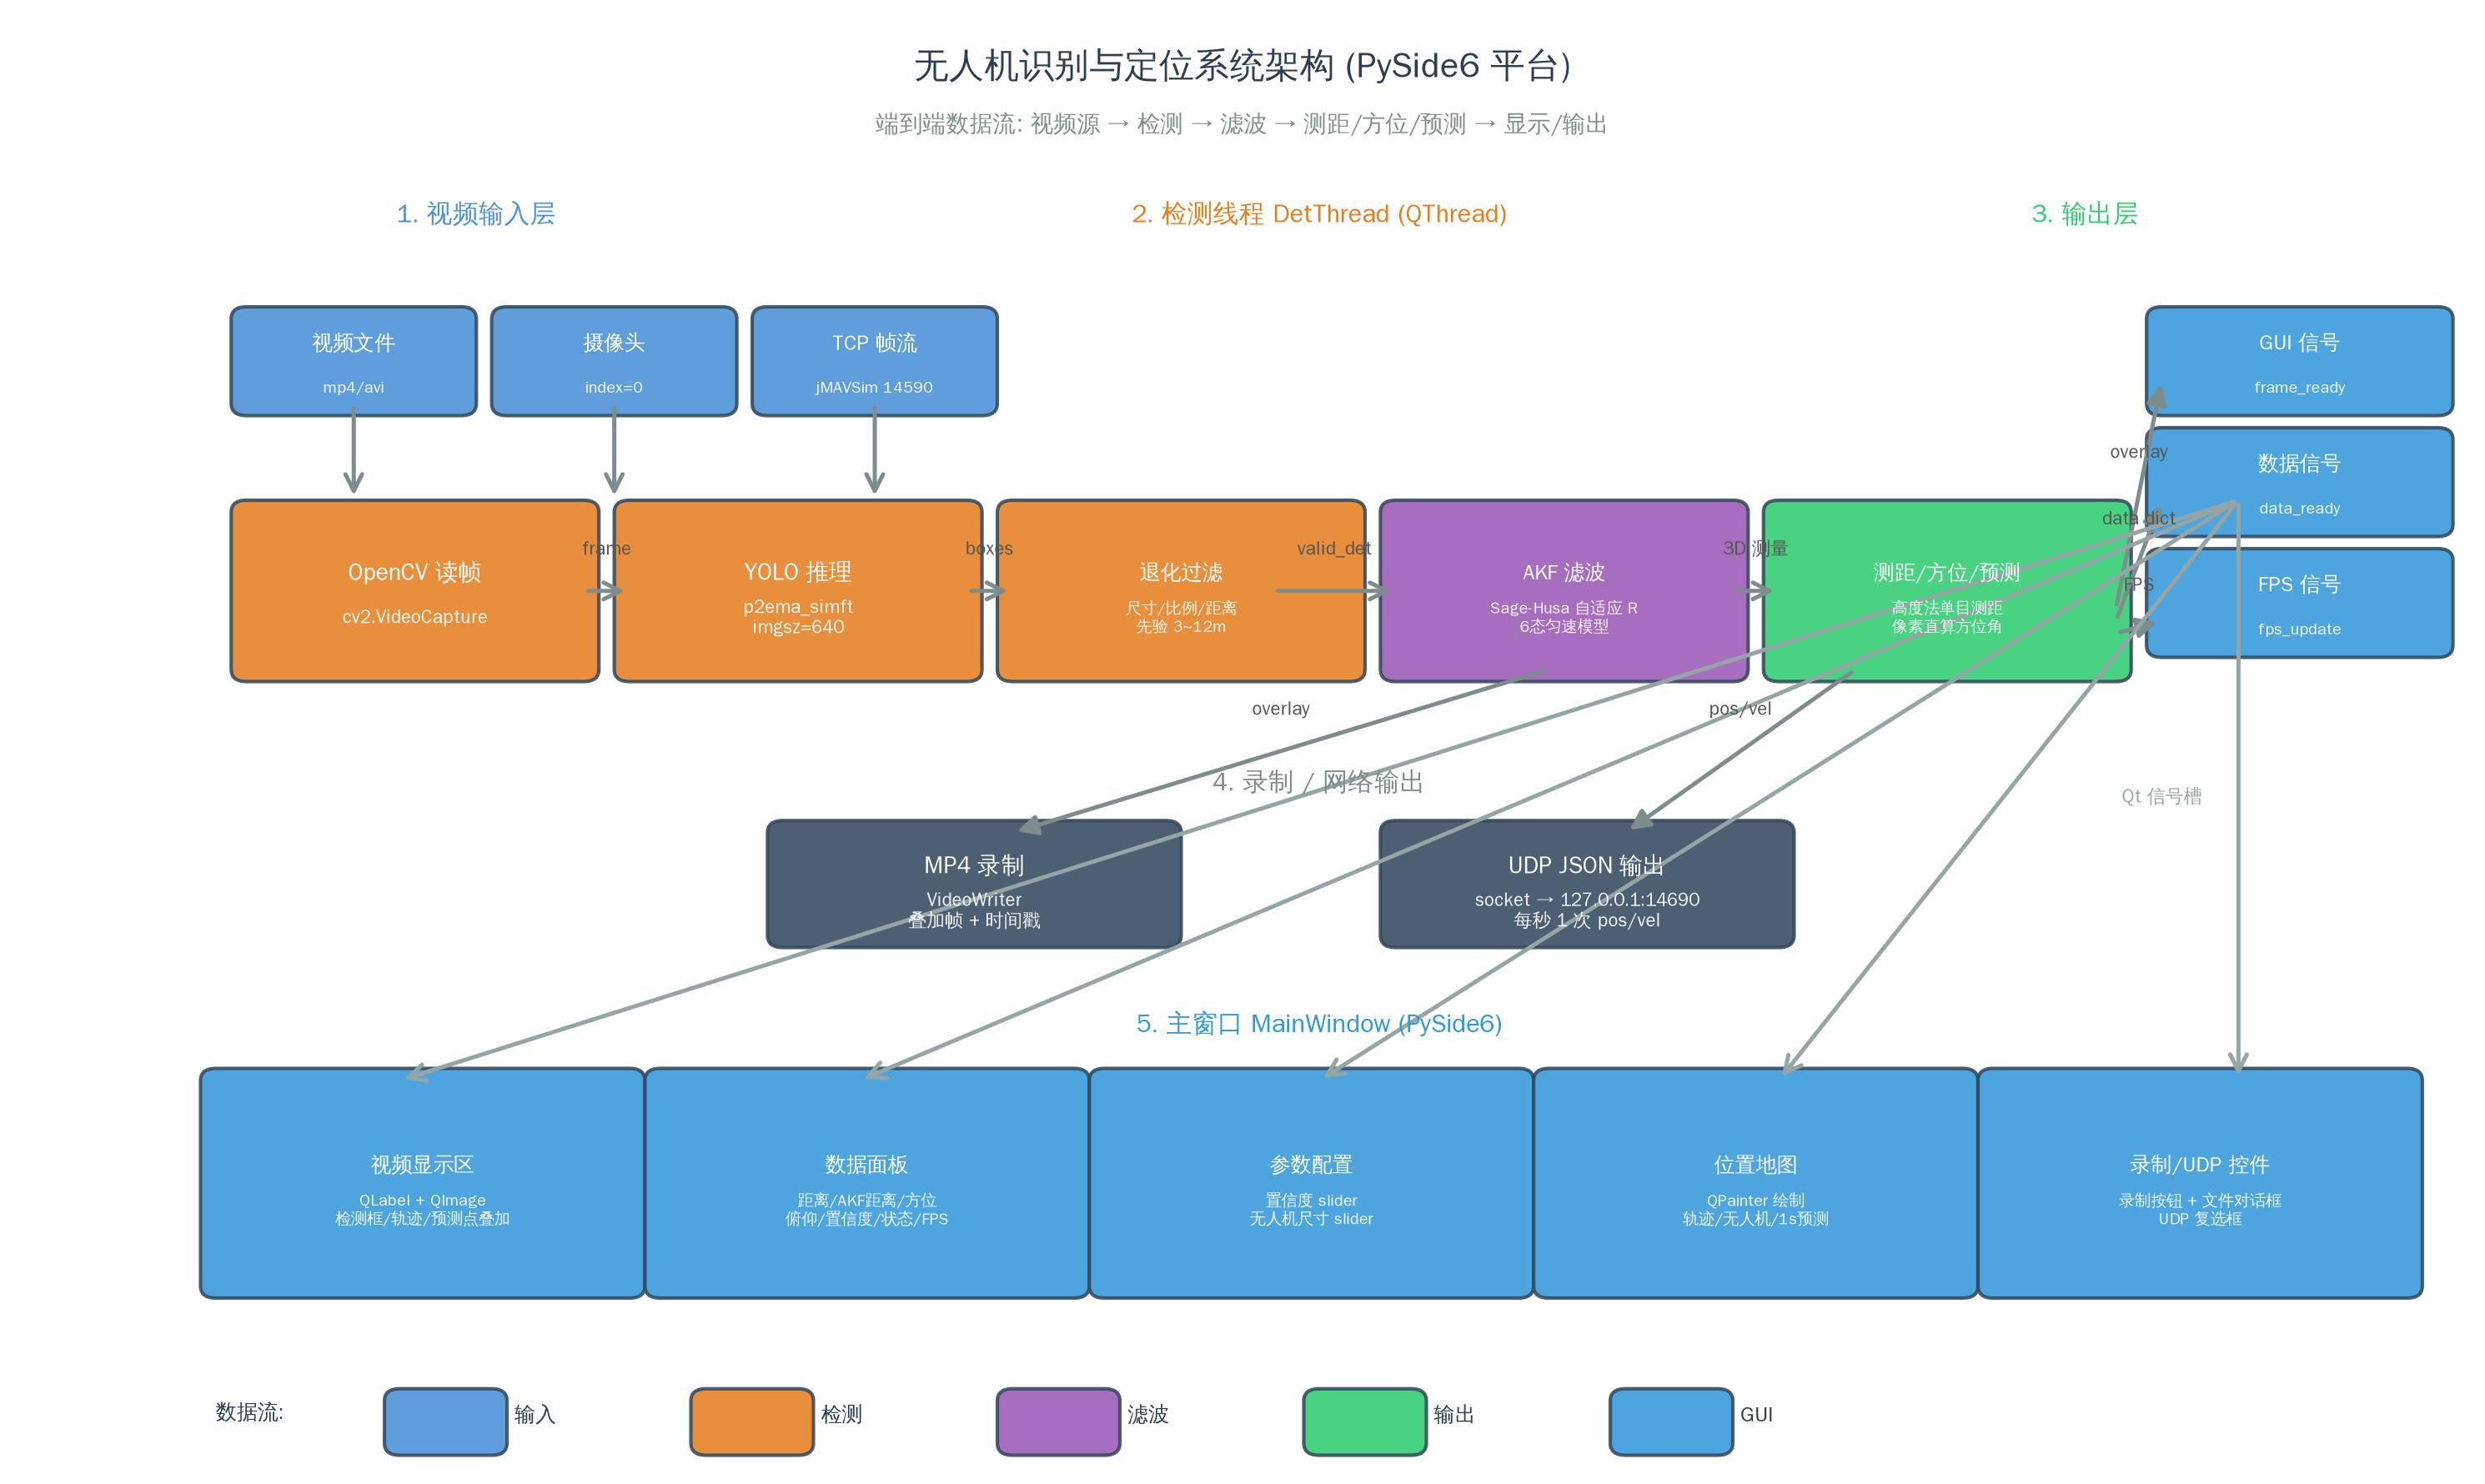
\includegraphics[width=0.95\textwidth]{images/pictures/system_arch.jpg}
\caption{系统总体架构}
\label{fig:sim_arch}
\end{figure}

数据流可以概括为四条链路：

\begin{itemize}
\item PX4 $\leftrightarrow$ jMAVSim：MAVLink，UDP 4560，双向；
\item jMAVSim $\rightarrow$ 算法端：护航相机视频帧，TCP 14590，30\,fps；
\item jMAVSim $\rightarrow$ 算法端：目标真值，UDP 14680 广播，50\,Hz；
\item 算法端 $\rightarrow$ 显示端：结构化结果，UDP/JSON 14690。
\end{itemize}

\subsection{lockstep 同步}

仿真启用 lockstep 模式。在该模式下，jMAVSim 每推进一个物理步都会等待 PX4 完成对应的控制计算，二者以相同的仿真时间前进，不会因为 CPU/GPU 负载波动而产生时间漂移。这对实验结果的可复现性至关重要：若没有 lockstep，仿真时间可能快于或慢于真实时间，导致 30\,fps 的视频流与 50\,Hz 的真值在时间上错位，进而影响测距与角度评估。

\subsection{启动流程}

闭环启动脚本按以下顺序执行：

（1）启动 PX4 SITL，加载多旋翼机型与默认参数；

（2）启动 jMAVSim，指定 TCP 端口、lockstep 与目标机标志；

（3）等待 PX4 与 jMAVSim 完成握手（jMAVSim 的 \texttt{Simulator} 构造函数会阻塞，直到收到第一条 MAVLink 消息）；

（4）启动算法端，连接 TCP 帧流并监听 UDP 真值；

（5）启动显示端，接收算法结果并渲染界面。

启动顺序不能颠倒：若 jMAVSim 先于 PX4 启动，会因等待握手而阻塞；若算法端先于帧流服务启动，会因连接失败而退出。本文通过启动脚本中的重试与等待逻辑保证顺序正确。

\section{jMAVSim 改造}

\subsection{改造需求}

原始 jMAVSim 仅支持单架由 PX4 控制的多旋翼，相机固定跟随该机，没有独立的"目标机"与"护航相机"，也不提供真值广播与视频推流。为构建反无人机仿真场景，本文提出以下改造需求：

（1）增加第二架由脚本控制的目标机，按预设航线飞行；

（2）增加一台独立的护航相机，始终注视目标机，模拟地面或伴飞观测平台；

（3）广播目标机真值（位置、速度、相机位置）供算法端评估；

（4）将护航相机画面编码为 JPEG 并通过 TCP 推送；

（5）支持纯离屏渲染，摆脱窗口系统依赖；

（6）构建城市级场景，包含建筑、树木、道路与广场。

\subsection{脚本目标机}

本文新增 \texttt{ScriptedQuad} 类，继承 \texttt{KinematicObject}，按时间参数化航迹更新位置与速度。航迹采用 Catmull-Rom 样条插值，在三维空域内生成 22 个航点。Catmull-Rom 样条的优点是曲线经过所有控制点，且切线连续，适合生成平滑的巡游路线。

设四个相邻控制点为 $\mathbf{P}_{i-1},\mathbf{P}_i,\mathbf{P}_{i+1},\mathbf{P}_{i+2}$，段参数 $t\in[0,1]$，则样条点为

\begin{equation}
\mathbf{C}(t) = \frac{1}{2}\Big[
2\mathbf{P}_i + (-\mathbf{P}_{i-1}+\mathbf{P}_{i+1})t
+ (2\mathbf{P}_{i-1}-5\mathbf{P}_i+4\mathbf{P}_{i+1}-\mathbf{P}_{i+2})t^2
+ (-\mathbf{P}_{i-1}+3\mathbf{P}_i-3\mathbf{P}_{i+1}+\mathbf{P}_{i+2})t^3
\Big].
\label{eq:catmull}
\end{equation}

对 $t$ 求导可得切线，用于确定飞行方向与速度方向：

\begin{equation}
\mathbf{C}'(t) = \frac{1}{2}\Big[
(-\mathbf{P}_{i-1}+\mathbf{P}_{i+1})
+ 2(2\mathbf{P}_{i-1}-5\mathbf{P}_i+4\mathbf{P}_{i+1}-\mathbf{P}_{i+2})t
+ 3(-\mathbf{P}_{i-1}+3\mathbf{P}_i-3\mathbf{P}_{i+1}+\mathbf{P}_{i+2})t^2
\Big].
\label{eq:catmull_deriv}
\end{equation}

航点范围经过设计，使目标始终处于护航相机的有效视野与检测距离内：$x\in[-9,9]$\,m，$y\in[-38.5,-29.5]$\,m，$z\in[-16,-9.5]$\,m（NED，负值表示高度）。每段速度为 0.8--2.8\,m/s，段内做加减速（见第~\ref{sec:formation} 节）。

\subsection{护航相机}

本文新增 \texttt{CameraRig} 类，同样继承 \texttt{KinematicObject}。与原始 jMAVSim 的固定相机不同，CameraRig 每帧读取目标机的实际位置与速度，计算期望机位，并以一阶低通的方式收敛。具体设计见第~\ref{sec:formation} 节。

护航相机的视场角设为 60\textdegree（水平），对应 1280 宽图像的焦距

\begin{equation}
f = \frac{W/2}{\tan(\mathrm{FOV}_h/2)} = \frac{640}{\tan30^{\circ}}\approx1108.5\ \text{px}.
\label{eq:fx}
\end{equation}

该焦距与算法端的测距公式一致，保证仿真与实拍的参数含义相同。

\subsection{真值广播}

本文新增 \texttt{TruthBroadcaster} 线程，以 50\,Hz 向 UDP 端口 14680 广播文本报文，格式为

\begin{verbatim}
t=<ms> tp=<x,y,z> tv=<vx,vy,vz> ep=<x,y,z> cp=<x,y,z>
\end{verbatim}

其中 \texttt{t} 为仿真时间戳，\texttt{tp} 为目标位置，\texttt{tv} 为目标速度，\texttt{ep} 为自身机位置，\texttt{cp} 为相机位置。坐标系为 NED，单位为米、米每秒。算法端按时间戳对齐视频帧与真值：由于帧流与真值流是两条独立的链路，必须用时间戳而非"收到顺序"对齐，否则会引入几十毫秒的偏差。

\subsection{离屏渲染与帧流}

原始 jMAVSim 依赖 Java3D 的窗口画布。在 WSL 环境中，窗口系统可能因 WSLg 的共享内存问题而不稳定，长时间运行会出现画面空白甚至进程崩溃。本文实现了纯离屏渲染：

（1）创建离屏 \texttt{Canvas3D}，不绑定到任何 \texttt{Frame}；

（2）每帧调用 \texttt{render} 将场景绘制到离屏缓冲区；

（3）用 \texttt{ImageIO} 将缓冲区编码为 JPEG；

（4）通过 TCP 连接推送"头部行 + 二进制数据"。

头部行格式为

\begin{verbatim}
<seq> <timestamp_ms> <width> <height> <nbytes>
\end{verbatim}

接收端先读取一行文本，解析出字节数，再精确读取相应长度的 JPEG 数据。这一协议避免了 TCP 粘包问题，也便于接收端检测丢帧（通过序号跳变）。

需要说明的是，离屏渲染必须关闭窗口画布的 \texttt{glXSwapBuffers} 调用，否则在软件渲染下会触发 JVM 崩溃；同时，离屏渲染不会因窗口最小化而暂停，保证帧流的连续性。

\subsection{场景构建}

本文新增 \texttt{SceneBuilder}、\texttt{SceneBuilding}、\texttt{SceneTree} 等类，以程序化方式构建城市场景。场景包含：

（1）\textbf{地面}：大范围草地纹理，中央铺设 140$\times$110\,m 的浅灰水泥广场，覆盖整条巡游轨迹，保证目标下方材质与地图显示一致；

（2）\textbf{建筑}：53 栋建筑，分布在目标飞行走廊两侧，高度均低于 8\,m，避免遮挡目标检测；建筑立面使用程序化贴图，按楼层与开间重复，色调压暗，避免"白色盒子"的卡通感；

（3）\textbf{树木}：82 棵近景树与 90 棵远景树，近景树冠由 6 个错位椭球堆叠而成，远景树线用于收拢地平线；

（4）\textbf{天空}：2048$\times$1024 的蓝天白云全景贴图，替换原始 jMAVSim 自带的公园照片背景。

场景对象总数约 149 个。所有建筑与树木的位置经过检查，确保不进入护航相机与目标机之间的视线通道。

\section{检测死区的发现}

\subsection{初期现象}

在闭环测试初期，本文使用 Det-Fly 训练的 YOLOv8n-P2-EMA 模型直接处理仿真画面，发现检测性能远低于验证集指标：模型在部分时段完全无响应，在部分时段只能间歇检出，且检出时段集中在特定距离。为量化这一现象，本文录制了 2228 帧（约 89.9\,s）的完整闭环视频，逐帧记录检测结果与真值。

\subsection{距离分层统计}

按真值距离对帧进行分层，统计各距离区间的检出率，结果如表~\ref{tab:deadzone} 所示。

\begin{table}[htbp]
\centering
\caption{微调前检测死区的距离分布（2228 帧）}
\label{tab:deadzone}
\small
\begin{tabular}{lccc}
\toprule
\textbf{距离区间(m)} & \textbf{检出率} & \textbf{主要表现} & \textbf{判定} \\
\midrule
3--4 & 0.0\% & 置信度接近 0 & 完全盲区 \\
4--5 & 0.0\% & 置信度接近 0 & 完全盲区 \\
5--6 & 5.8\% & 偶发弱响应 & 近乎盲区 \\
6--7 & 7.4\% & 弱响应 & 近乎盲区 \\
7--8 & 39.0\% & 可检出但不稳定 & 有效窗口 \\
8--9 & 29.3\% & 可检出但不稳定 & 有效窗口 \\
9--10 & 0.0\% & 仅弱响应，低于初锁门限 & 无法锁定 \\
\bottomrule
\end{tabular}
\end{table}

由表可见，模型的有效工作窗口仅为 7--9\,m，窗口两侧均为死区。全帧检出率仅 10.0\%，与验证集 83.5\% 的 mAP50 形成鲜明对比。

进一步地，本文对 1793 个纯搜索帧做了三态划分：

（1）\textbf{真盲帧}：最高置信度低于 0.25，共 1454 帧，占 81.1\%；

（2）\textbf{弱响应帧}：最高置信度在 0.25--0.55 之间，共 270 帧，占 15.1\%；

（3）\textbf{先验拒绝帧}：最高置信度超过 0.55，但距离超出 3--12\,m 先验空域，被空间约束剔除，共 69 帧，占 3.8\%。

这说明死区的主要表现不是"检测到但被门限拒绝"，而是"根本没有有效响应"。

\begin{figure}[htbp]
\centering
\subfloat[近距离盲区帧（目标占画面比例大）]{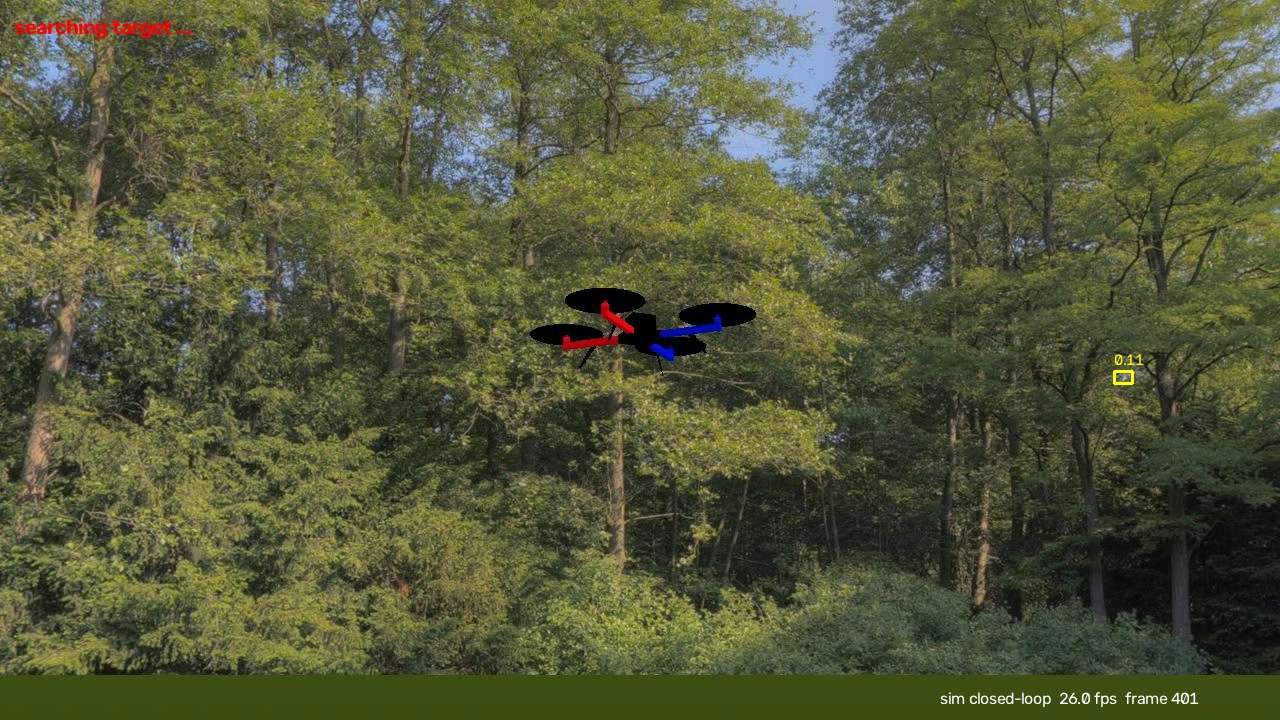
\includegraphics[width=0.47\textwidth]{images/pictures/deadzone_frame1.jpg}}
\hfill
\subfloat[有效窗口帧]{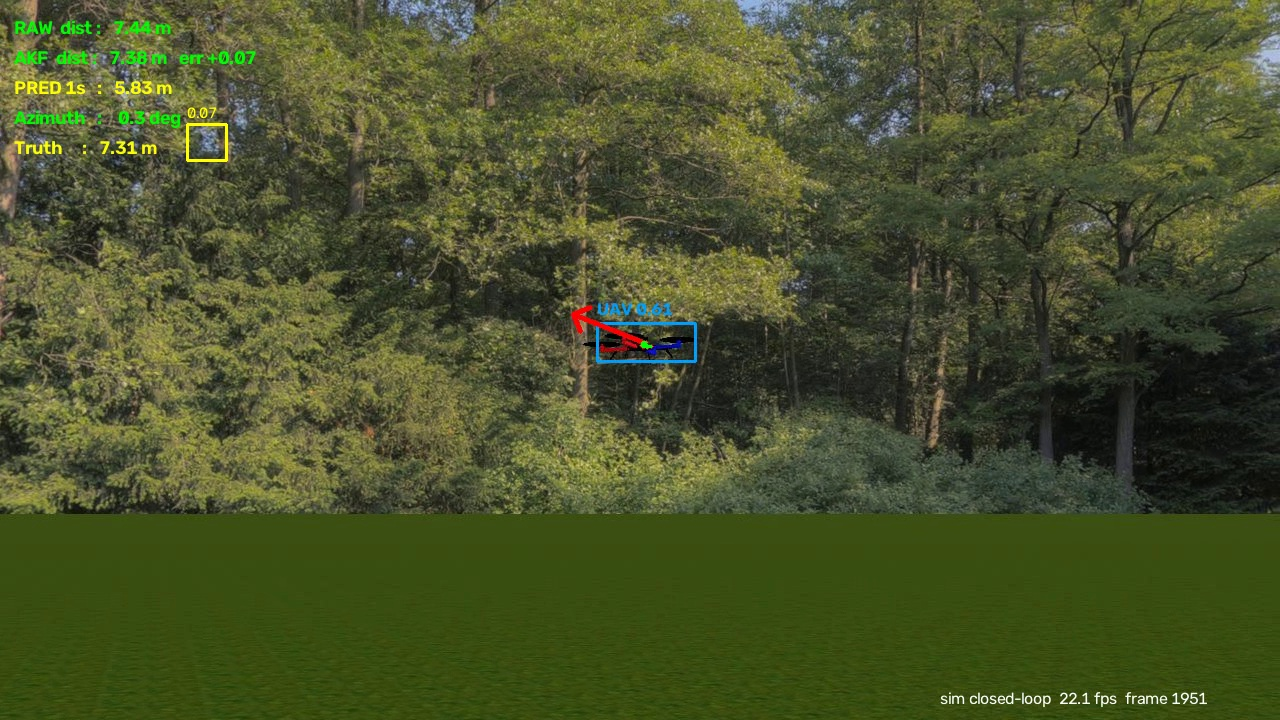
\includegraphics[width=0.47\textwidth]{images/pictures/deadzone_frame2.jpg}}
\caption{死区帧与有效帧对比}
\label{fig:deadzone_frames}
\end{figure}

\subsection{排除视角假设}

面对"近距离完全无响应"的现象，第一反应是"相机俯视目标导致失效"。本文对此假设做了定量检验。利用真值几何，计算每一帧中相机到目标的俯仰角（depression angle），并比较锁定帧与盲帧的分布：

（1）锁定帧的俯仰角中位数为 $-7.6$\textdegree；

（2）盲帧的俯仰角中位数为 $-5.4$\textdegree。

两者的差异仅 2.2\textdegree，且方向与"俯视导致失效"的预期相反（盲帧更接近水平）。这说明视角不是决定因素。进一步检查发现，目标飞行高度约 12--13\,m，护航相机高度约 12\,m，二者基本同高，根本不存在明显俯视。至此，视角假设被定量证伪。

\subsection{尺度分布解释}

排除视角后，本文将注意力转向目标在画面中的尺度。统计表明，死区与距离高度相关，而距离直接决定目标在画面中的像素尺寸。在 3--6\,m 时，目标高度可达画面的 1/5 至 1/3，远超 Det-Fly 的远距小目标分布；在 9\,m 以上时，目标高度不足画面的 1/20，信息量不足以支撑稳定检出。模型在训练中从未见过如此大的目标，将其视为"背景中的未知物体"，输出置信度接近 0。

这一解释可以用分布外（Out-of-Distribution，OOD）检测的理论理解：模型的特征提取器在训练分布内具有判别力，一旦输入落在分布外，网络的响应会变得不可预测，常见表现是置信度崩塌。本文的近距离样本正是典型的 OOD 输入。

\subsection{对系统设计的影响}

死区的存在意味着：即使检测模型在公开数据集上指标优秀，也不能保证在特定部署场景中可用。系统设计必须包含"部署域验证"环节，通过少量目标域数据检查模型的实际工作范围。本文的处理方式是仿真域微调，但更一般的工程做法是：在部署前采集目标场景的少量样本，评估检出率随距离/尺度的变化，再决定是否需要微调或调整镜头焦距。

\section{仿真域微调}

\subsection{数据采集与自动标注}

微调数据的构建方法已在第三章详细介绍。简单回顾：利用护航相机注视目标的特性，将框中心约束在光轴附近，由真值距离与等效尺寸反算框高，共采集 450 帧，按距离分层覆盖 3--12\,m。标注过程无人工介入，避免了标注成本与主观误差。

\subsection{微调配置}

微调在 Det-Fly 预训练权重的基础上进行，关键参数如表~\ref{tab:finetune_hp} 所示。

\begin{table}[htbp]
\centering
\caption{仿真域微调超参数}
\label{tab:finetune_hp}
\small
\begin{tabular}{lc}
\toprule
\textbf{参数} & \textbf{取值} \\
\midrule
初始化权重 & p2ema\_v8n（Det-Fly 训练） \\
训练轮次 & 20 \\
初始学习率 & 0.001 \\
批量大小 & 8 \\
输入尺寸 & 640$\times$640 \\
Mosaic & 关闭 \\
混合精度 & 开启 \\
训练/验证划分 & 360/90（按飞行段划分） \\
\bottomrule
\end{tabular}
\end{table}

关闭 Mosaic 的原因已在第三章说明：仿真数据的尺度分布是分层设计的，Mosaic 会破坏这一分布。学习率取 0.001，低于从头训练的 0.01，目的是在保留预训练特征的同时做温和的域适应，避免灾难性遗忘。

\subsection{微调结果}

微调前后的对比结果如表~\ref{tab:finetune_result} 所示。

\begin{table}[htbp]
\centering
\caption{仿真域微调前后对比}
\label{tab:finetune_result}
\small
\begin{tabular}{lcc}
\toprule
\textbf{指标} & \textbf{微调前} & \textbf{微调后} \\
\midrule
3--10\,m 全段检出率 & 10.0\%--11.5\% & \textbf{100.0\%} \\
有效工作窗口 & 7--9\,m & 3--10\,m（全覆盖） \\
置信度中位数 & 接近 0 & 0.867 \\
置信度最小值 & -- & 0.805 \\
AKF 稳态中位误差 & 0.44\,m & \textbf{0.13\,m} \\
稳态帧占比 & 7\% & \textbf{99.8\%} \\
方位角误差中位 & 0.21\textdegree & \textbf{0.05\textdegree} \\
俯仰角误差中位 & 0.88\textdegree & 0.93\textdegree \\
等效尺寸 & 0.230\,m & 0.270\,m \\
\bottomrule
\end{tabular}
\end{table}

\begin{figure}[htbp]
\centering
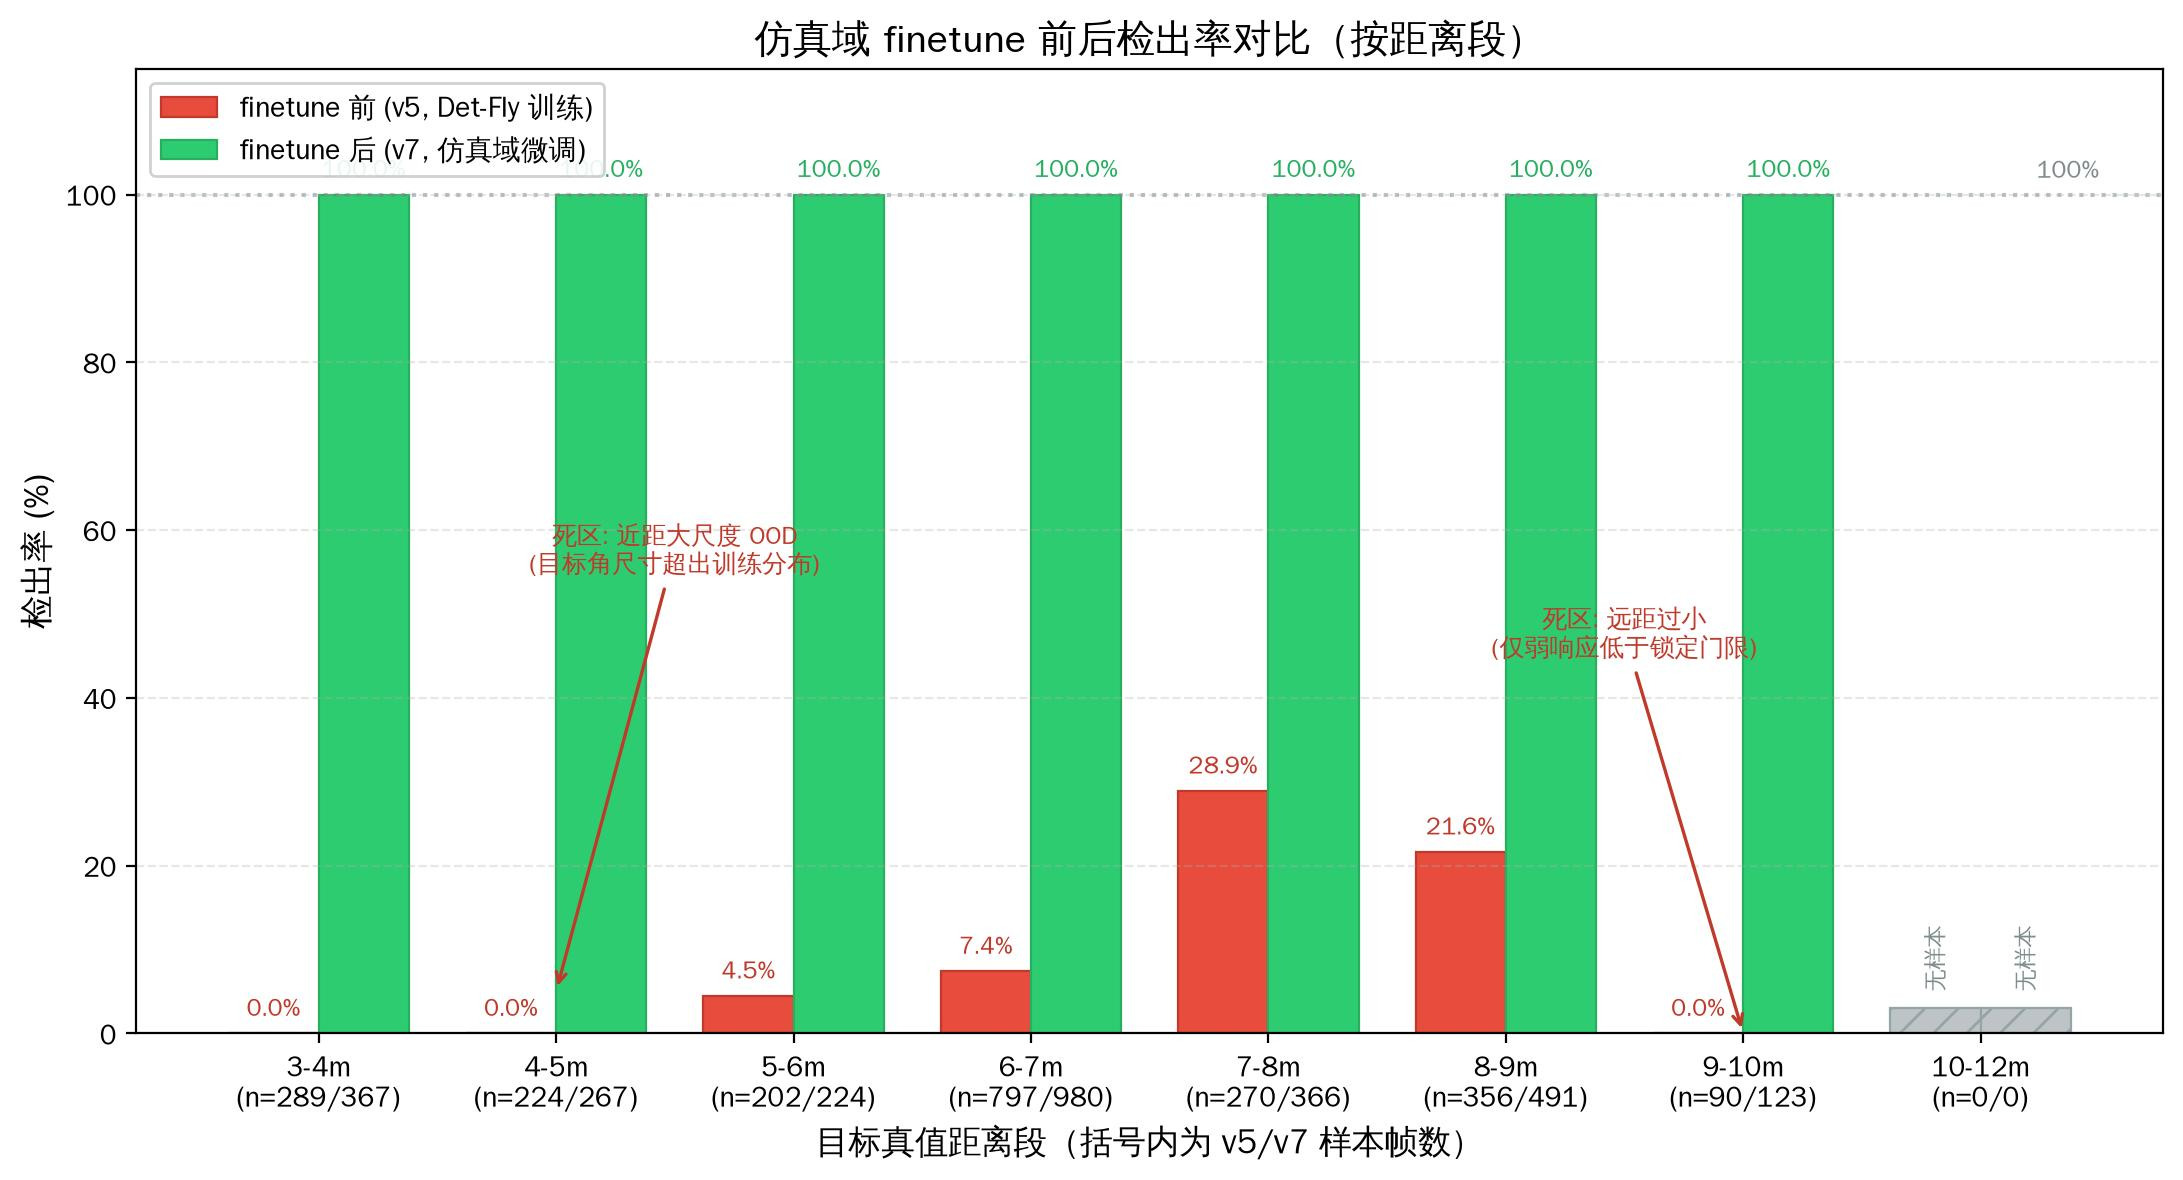
\includegraphics[width=0.92\textwidth]{images/pictures/deadzone_before_after.jpg}
\caption{微调前后的检测死区对比}
\label{fig:deadzone_ba}
\end{figure}

微调后，3--10\,m 全距离段检出率达到 100\%，置信度中位数 0.867、最小值 0.805，均远高于 0.55 的初锁门限。AKF 稳态中位误差从 0.44\,m 降至 0.13\,m，稳态帧占比从 7\% 提升至 99.8\%。这些结果表明，仿真域微调不仅消除了死区，还显著改善了测距的稳定性。

需要如实说明的是：10--12\,m 区间在微调前的录像中没有足够的真实飞行样本，表~\ref{tab:deadzone} 中的"9--10\,m 0\%"不能外推为"10--12\,m 也必然为 0"。本文在数据采集中补充了 9--12\,m 的 120 帧，因此微调后该区间也有覆盖，但缺少独立的验证录像，相关结论应以"设计覆盖"而非"实测覆盖"表述。

\subsection{域适应的机理讨论}

为什么仅用 450 帧就能消除死区？本文认为有三点原因。

（1）\textbf{特征分布对齐}。Det-Fly 训练的特征提取器已经学会了"无人机"的一般外观，但仿真渲染的边缘、光照与噪声分布不同。少量仿真数据足以让网络调整浅层卷积的响应，使仿真目标落入已有特征的可判别区域。

（2）\textbf{尺度分布补齐}。450 帧按距离分层，重点补充了近距离大尺度与远距离小尺度样本，直接填补了训练分布的空白。这是死区消除的关键。

（3）\textbf{微调强度适中}。学习率 0.001、20 轮、关闭 Mosaic，使模型在适应新域的同时保留了原有能力。若学习率过大或训练过久，模型可能过拟合到仿真域，在真实数据上反而退化。本文在实测中也观察到：微调模型在实拍视频上的检出率高于未微调模型（见第九章），说明适度的仿真域微调具有一定的泛化收益。

\section{编队巡游与尾随相机}
\label{sec:formation}

\subsection{设计目标}

早期仿真中，目标机与相机各自沿独立路径运动，二者之间没有明确的"主动—被动"关系，画面看起来像"相机吸附在目标上"或"目标追着相机飞"，缺乏真实监视场景中的追踪感。为更真实地模拟"地面/伴飞平台追踪目标"的场景，本文实现了编队巡游与尾随相机：

（1）目标机是主动飞行方，按预设航线飞行并做加减速；

（2）相机是被动追随方，根据目标的实际位置与速度计算期望机位，带滞后地跟随；

（3）相机瞄准一个"滞后于目标"的瞄准点，使目标在画面中自然漂移，而不是死锁在中心。

\subsection{目标机航迹与加减速}

目标机的航迹由两部分叠加：局部样条航迹与全局编队偏移。局部样条航迹定义在以相机为原点的局部空域内，保证检测距离在 3--10\,m；全局编队偏移将整段航迹"搬运"到城市的椭圆路线上：

\begin{equation}
n(a) = C_X + R_X\sin a,\qquad e(a) = C_Y + R_Y(1-\cos a),
\label{eq:ellipse}
\end{equation}

其中 $C_X=8$\,m、$C_Y=-4$\,m 为椭圆中心，$R_X=18$\,m、$R_Y=22$\,m 为半轴，$a$ 为随速度累加的角度参数。椭圆周长约 126\,m，以 2\,m/s 巡游约 63\,s 一圈。

为体现真实飞行的加减速，本文对每段参数 $t$ 做 smoothstep 重参数化：

\begin{equation}
u = (1-\gamma)t + \gamma\,t^2(3-2t),\qquad
\frac{du}{dt} = (1-\gamma)+\gamma\cdot6t(1-t),
\label{eq:smoothstep}
\end{equation}

其中 $\gamma=0.75$ 为变速强度。端点处 $du/dt=1-\gamma=0.25$，即速度降至段均速的 25\%（减速过弯）；中点处 $du/dt=1-\gamma+1.5\gamma=1.375$，即速度升至段均速的 137.5\%（加速出弯）。速度向量按切线方向乘以 $du$ 计算：

\begin{equation}
\mathbf{v} = \frac{\mathbf{C}'(u)}{\|\mathbf{C}'(u)\|}\cdot v_{seg}\cdot\frac{du}{dt}.
\label{eq:velocity}
\end{equation}

这样，真值广播中的速度与目标实际运动一致，便于评估速度对检测与测距的影响。实测速度在 0.21--2.95\,m/s 之间连续变化，不再是人造匀速。

\subsection{尾随相机动力学}

相机的期望机位定义为沿目标速度反方向、距离 $d$ 处，并略低于目标：

\begin{equation}
\mathbf{p}_{des} = \mathbf{p}_{t} - \hat{\mathbf{v}}_{t}^{xy}\cdot d + \begin{bmatrix}0\\0\\\Delta z\end{bmatrix},
\label{eq:cam_desired}
\end{equation}

其中 $\hat{\mathbf{v}}_t^{xy}$ 为目标水平速度的单位方向，$\Delta z=1.2$\,m（NED 下为正，表示相机低于目标 1.2\,m，形成轻微仰视，检测模型在侧视/仰视下更稳定）。距离 $d$ 随目标速度"呼吸"：

\begin{equation}
d = d_0 + \min\left(k_v\|\mathbf{v}_t^{xy}\|,\,d_{max}\right),
\label{eq:cam_dist}
\end{equation}

本文取 $d_0=5.0$\,m、$k_v=0.5$\,s、$d_{max}=1.0$\,m，即速度每增加 2\,m/s，相机后退 1\,m，最大额外距离 1\,m。

相机位置不是直接设置为期望机位，而是以时间常数 $\tau=0.6$\,s 做一阶低通：

\begin{equation}
\mathbf{p}_{c,k} = \mathbf{p}_{c,k-1} + \left(1-e^{-\Delta t/\tau}\right)\left(\mathbf{p}_{des,k}-\mathbf{p}_{c,k-1}\right).
\label{eq:cam_lpf}
\end{equation}

这一滞后是"追踪感"的来源：目标转弯时，相机需要时间才能转到新的尾随方向，画面中目标会先偏向一侧，随后被"追回"；目标加速时，相机被甩开，距离暂时增大，随后收敛。

\subsection{瞄准点滞后}

若相机直接对准目标本体，目标将始终位于画面中心，看起来像"吸附"。本文引入瞄准点（AimPoint）：它是目标位置的低通滞后副本，

\begin{equation}
\mathbf{p}_{aim,k} = \mathbf{p}_{aim,k-1} + \left(1-e^{-\Delta t/\tau_{aim}}\right)\left(\mathbf{p}_{t,k}-\mathbf{p}_{aim,k-1}\right),
\label{eq:aim}
\end{equation}

其中 $\tau_{aim}=0.45$\,s。相机对准 $\mathbf{p}_{aim}$ 而非 $\mathbf{p}_t$，于是目标在画面中会自然漂移：目标领先于瞄准点时，出现在画面中心前方；目标转向时，出现在画面一侧。这种漂移与真实监视画面中"操作员手动跟踪、目标略微偏离中心"的观感一致。

\subsection{验证结果}

本文通过真值 UDP 抓包统计了尾随相机的实际距离与目标速度：

（1）距离：100 个样本，最小 5.22\,m，中位 5.29\,m，最大 5.41\,m；

（2）速度：120 个样本，最小 0.94\,m/s，中位 1.40\,m/s，最大 1.57\,m/s；另一轮长时统计为 0.21--2.95\,m/s。

距离稳定在 5.2--5.4\,m，处于检测模型的可靠工作区间；速度连续变化，体现了加减速。图~\ref{fig:dashboard_live} 给出了运行中的界面截图，可以看到目标在光电画面中略微偏离中心，符合尾随跟踪的观感。

\begin{figure}[htbp]
\centering
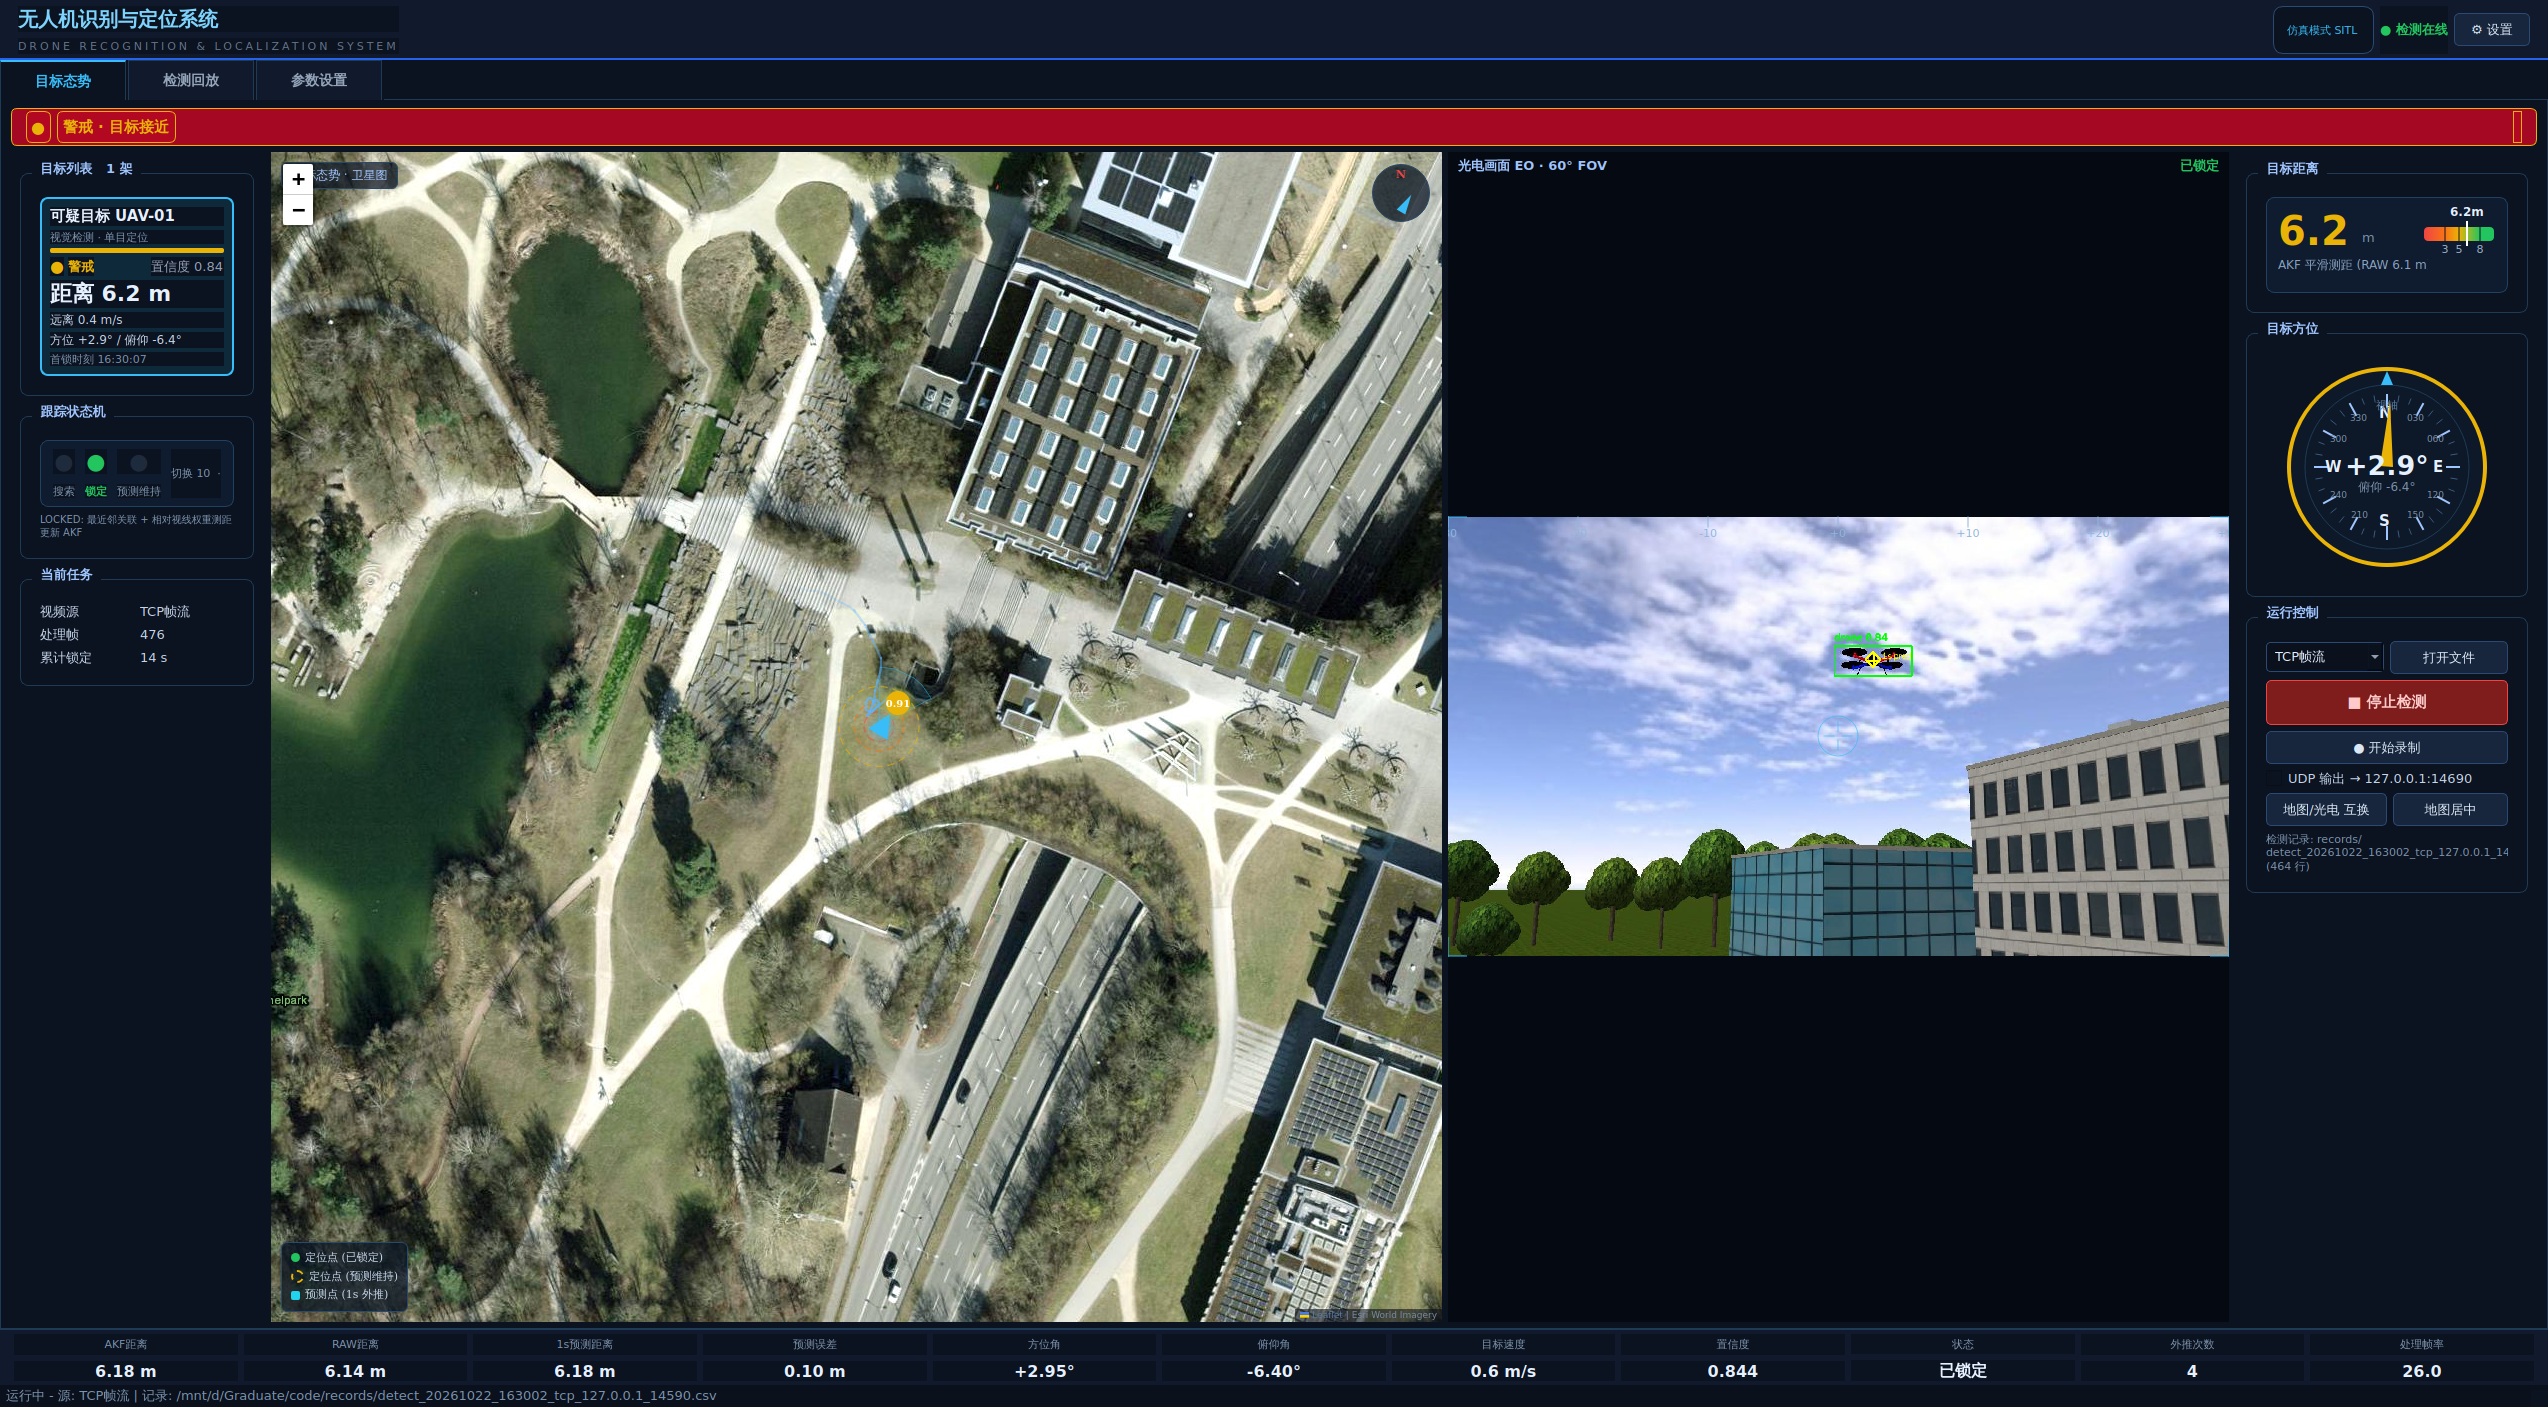
\includegraphics[width=0.95\textwidth]{images/pictures/dashboard_live.png}
\caption{编队巡游与尾随相机运行界面}
\label{fig:dashboard_live}
\end{figure}

\subsection{设计约束}

尾随相机的设计受检测模型的物理约束。实验表明，当相机俯视目标（目标低于相机 3--8\,m）时，检出率会从 73\%--77\% 降至 22\%--37\%，原因是俯视视角下目标投影变形、旋翼与机身重叠。因此本文让相机始终略低于目标（$\Delta z=1.2$\,m），保持轻微仰视。这一约束说明：仿真场景的设计不能只考虑"好看"，还必须服从算法的适用域。

\section{本章小结}

本章构建了完整的仿真闭环验证平台。在架构上，采用 PX4 SITL + jMAVSim + 算法端三进程结构，通过 lockstep 保证时间一致；在改造上，新增脚本目标机、护航相机、真值广播、离屏帧流与城市场景，解决了 WSL 环境下的窗口依赖问题；在分析上，通过 2228 帧的距离分层统计与真值几何审计，定量证伪了"俯视导致失效"的假设，将检测死区归因于目标尺度分布偏移；在方法上，提出零人工标注的仿真域微调，用 450 帧分层数据将 3--10\,m 检出率从约 10\% 提升至 100\%；在场景上，实现了目标机主动飞行、相机被动尾随的编队巡游与加减速行为，使仿真画面具备真实的追踪感。该平台为后续系统集成与实验评估提供了可复现的基础。
